\section{Cluster analysis}
\frame{\sectionpage}


\begin{frame}[fragile]{Cluster Analysis}

  \begin{itemize}
  \item One side-effect of discriminant analysis: could draw picture of data (if 1st 2s \texttt{LD}s told most of story) and see which individuals ``close'' to each other.
  \item Discriminant analysis requires knowledge of groups.
  \item Without knowledge of groups, use {\em cluster analysis}: see which individuals close, which groups suggested by data.
  \item Idea: see how individuals group into ``clusters'' of nearby individuals.
  \item Base on ``dissimilarities'' between individuals.
  \item Or base on standard deviations and correlations between variables (assesses dissimilarity behind scenes).
  \end{itemize}

\end{frame}

\begin{frame}[fragile]{Packages}
  
\begin{knitrout}
\definecolor{shadecolor}{rgb}{0.969, 0.969, 0.969}\color{fgcolor}\begin{kframe}
\begin{alltt}
\hlkwd{library}\hlstd{(tidyverse)}
\end{alltt}


{\ttfamily\noindent\itshape\color{messagecolor}{\#\# Loading tidyverse: ggplot2\\\#\# Loading tidyverse: tibble\\\#\# Loading tidyverse: tidyr\\\#\# Loading tidyverse: readr\\\#\# Loading tidyverse: purrr\\\#\# Loading tidyverse: dplyr}}

{\ttfamily\noindent\itshape\color{messagecolor}{\#\# Conflicts with tidy packages ----------------------------------------------}}

{\ttfamily\noindent\itshape\color{messagecolor}{\#\# filter(): dplyr, stats\\\#\# lag():\ \ \ \ dplyr, stats}}\begin{alltt}
\hlkwd{library}\hlstd{(MASS)} \hlcom{# for lda later}
\end{alltt}


{\ttfamily\noindent\itshape\color{messagecolor}{\#\# \\\#\# Attaching package: 'MASS'}}

{\ttfamily\noindent\itshape\color{messagecolor}{\#\# The following object is masked from 'package:dplyr':\\\#\# \\\#\#\ \ \ \  select}}\begin{alltt}
\hlkwd{library}\hlstd{(ggrepel)}
\end{alltt}
\end{kframe}
\end{knitrout}

  
\end{frame}

\begin{frame}[fragile]{One to ten in 11 languages}

  \begin{tabular}{lcccccc}
    & English & Norwegian & Danish & Dutch & German\\
    \hline
    1 & one & en & en & een & eins\\
    2 & two & to & to & twee & zwei\\
    3 & three & tre & tre & drie & drei\\
    4 & four & fire & fire & vier & vier\\
    5 & five & fem & fem & vijf & funf\\
    6 & six & seks & seks & zes & sechs\\
    7 & seven & sju & syv & zeven & sieben\\
    8 & eight & atte & otte & acht & acht\\
    9 & nine & ni & ni & negen & neun\\
    10 & ten & ti & ti & tien & zehn\\
    \hline
    \end{tabular}
\end{frame}

\begin{frame}[fragile]{One to ten}

  \begin{tabular}{lcccccc}

    & French & Spanish & Italian & Polish & Hungarian & Finnish\\
\hline
    1 & un & uno & uno & jeden & egy & yksi\\
    2 & deux & dos & due & dwa & ketto & kaksi\\
    3 & trois & tres & tre & trzy &  harom & kolme\\
    4 & quatre & cuatro & quattro & cztery & negy & nelja\\
    5 & cinq & cinco & cinque & piec & ot & viisi\\
    6 & six & seis & sei & szesc & hat & kuusi\\
    7 & sept & siete & sette & siedem & het & seitseman \\
    8 & huit & ocho & otto & osiem & nyolc & kahdeksan\\
    9 & neuf & nueve & nove & dziewiec & kilenc & yhdeksan \\
    10 & dix & diez & dieci & dziesiec & tiz & kymmenen\\
    \hline
  \end{tabular}

\end{frame}


\begin{frame}[fragile]{Dissimilarities and languages example}

  \begin{itemize}
  \item Can define dissimilarities how you like (whatever makes sense in application).
  \item Sometimes defining ``similarity'' makes more sense; can turn this into dissimilarity by subtracting from some maximum.
  \item Example: numbers 1--10 in various European languages. Define
    similarity between two languages by counting how often the same
    number has a name starting with the same letter (and dissimilarity
    by how often number has names starting with different letter).
  \item Crude (doesn't even look at most of the words), but see how effective.
  \end{itemize}
  
\end{frame}

\begin{frame}[fragile]{Two kinds of cluster analysis}

  \begin{itemize}
  \item Looking at process of forming clusters (of similar languages):
    \textbf{hierarchical cluster analysis} (\texttt{hclust}).
    \begin{itemize}
    \item Start with each individual in cluster by itself.
    \item Join ``closest'' clusters one by one until all individuals in one cluster.
    \item How to define closeness of two \emph{clusters}? Not obvious,
      investigate in a moment.
    \end{itemize}
  \item Know how many clusters: which division into that many clusters
    is ``best'' for individuals? \textbf{K-means clustering} (\texttt{kmeans}).
  \end{itemize}
  
\end{frame}

\begin{frame}[fragile]{Two made-up clusters}
  
\begin{knitrout}
\definecolor{shadecolor}{rgb}{0.969, 0.969, 0.969}\color{fgcolor}
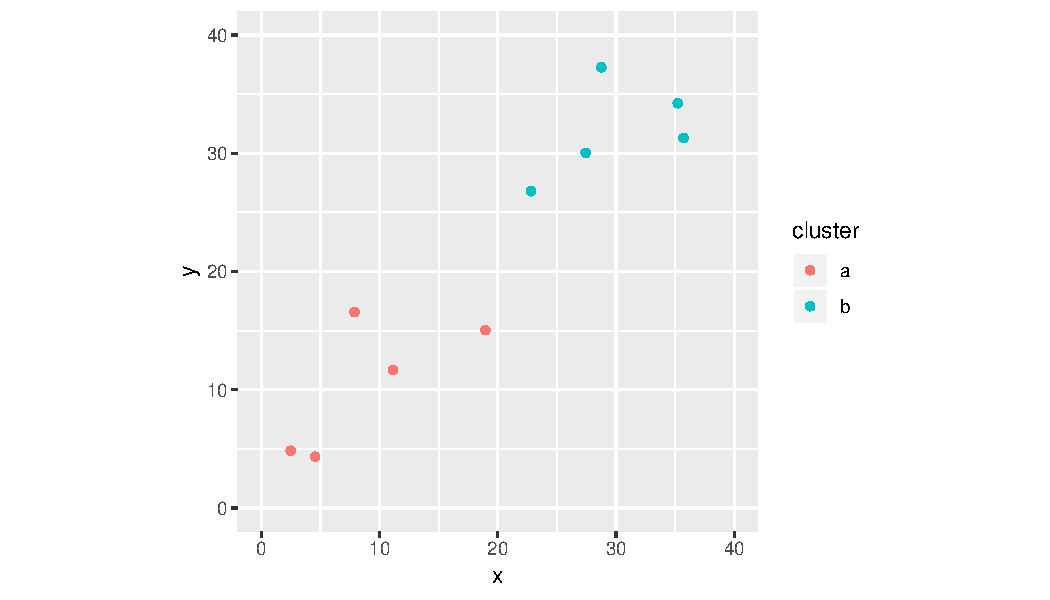
\includegraphics[width=\maxwidth]{figure/unnamed-chunk-2-1} 

\end{knitrout}

How to measure distance between set of red points and set of blue
ones? 
  
\end{frame}

\begin{frame}[fragile]{Single-linkage distance}
  
  Find the red point and the blue point that are closest together:
  
\begin{knitrout}
\definecolor{shadecolor}{rgb}{0.969, 0.969, 0.969}\color{fgcolor}
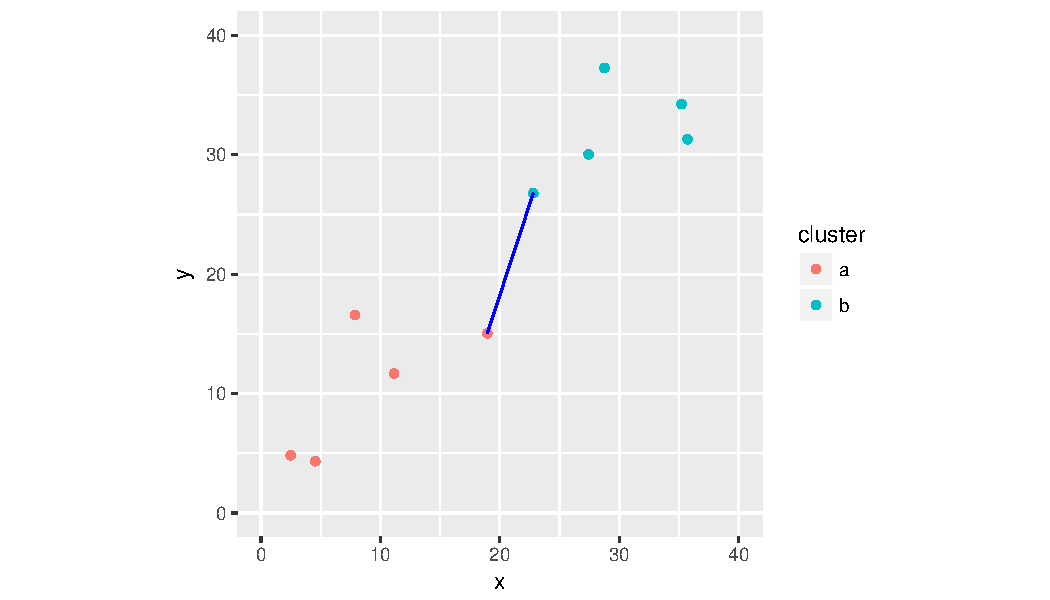
\includegraphics[width=\maxwidth]{figure/unnamed-chunk-3-1} 

\end{knitrout}

Single-linkage distance between 2 clusters is distance between their
closest points.
  
\end{frame}

\begin{frame}[fragile]{Complete linkage}
  
  Find the red and blue points that are farthest apart:
  
\begin{knitrout}
\definecolor{shadecolor}{rgb}{0.969, 0.969, 0.969}\color{fgcolor}
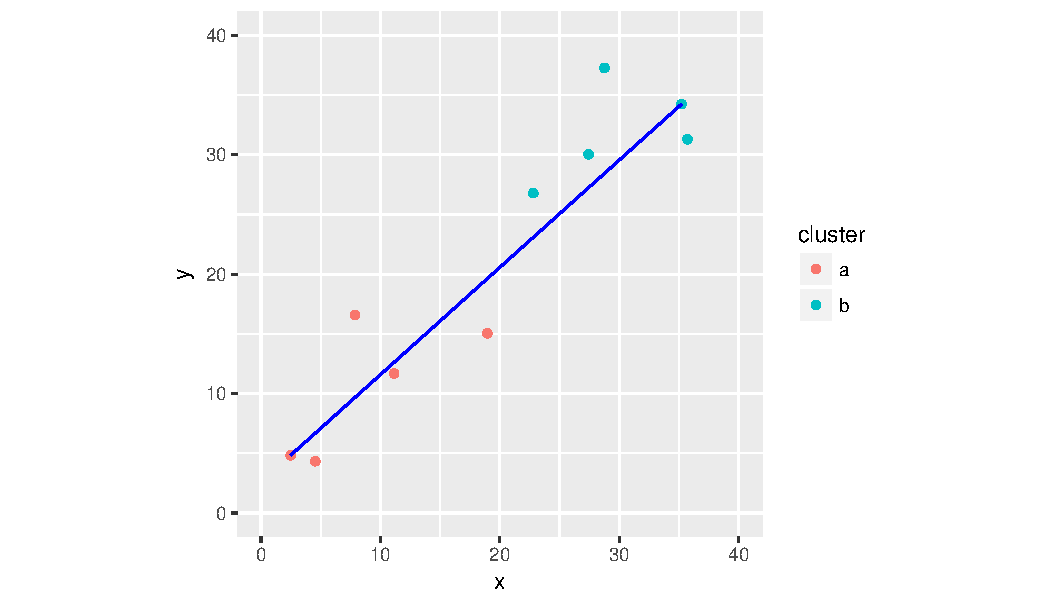
\includegraphics[width=\maxwidth]{figure/unnamed-chunk-4-1} 

\end{knitrout}

Complete-linkage distance is distance between farthest points. 
  
\end{frame}

\begin{frame}[fragile]{Ward's method}
  
  Work out mean of each cluster and join point to its mean:
  
\begin{knitrout}
\definecolor{shadecolor}{rgb}{0.969, 0.969, 0.969}\color{fgcolor}
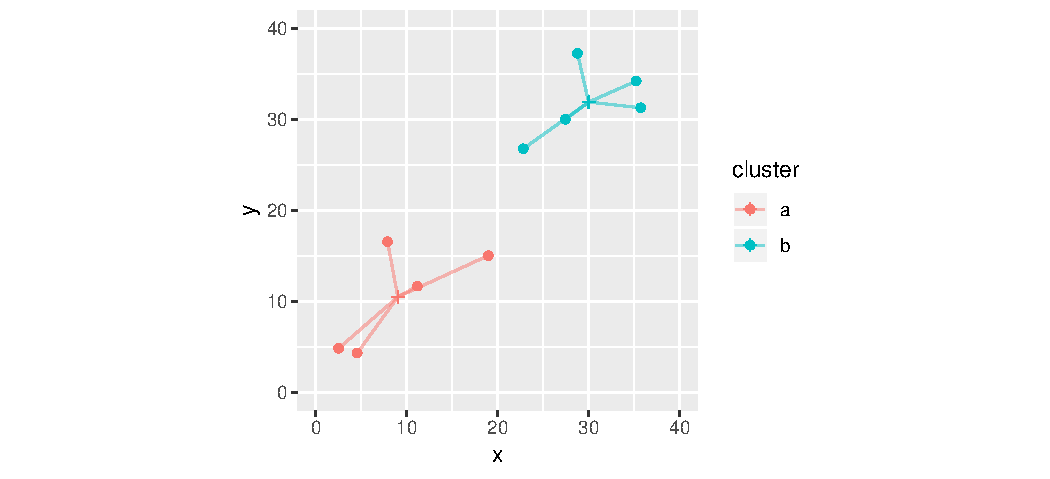
\includegraphics[width=\maxwidth]{figure/unnamed-chunk-5-1} 

\end{knitrout}

(i) Work out sum of squared distances of points from means.
\end{frame}

\begin{frame}[fragile]{Ward's method part 2}
  
Now imagine combining the two clusters and working out overall
mean. Join each point to this mean:

\begin{knitrout}
\definecolor{shadecolor}{rgb}{0.969, 0.969, 0.969}\color{fgcolor}
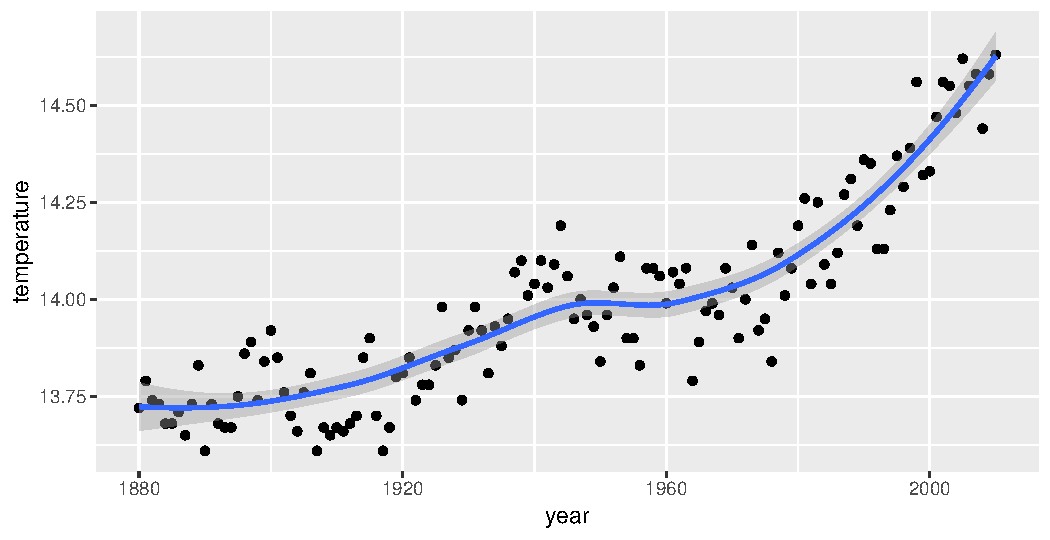
\includegraphics[width=\maxwidth]{figure/unnamed-chunk-6-1} 

\end{knitrout}
(ii) Calc sum of squared distances of points to combined mean.
  
\end{frame}

\begin{frame}[fragile]{Ward's method part 3}
  
  \begin{itemize}
  \item (ii) will be bigger than (i) (points closer to own cluster
    mean than combined mean).
  \item Ward's distance is (ii) minus (i).
  \item Think of as ``cost'' of combining clusters:
    \begin{itemize}
    \item if clusters close together, (ii) only a little larger than
      (i)
    \item if clusters far apart, (ii) a lot larger than (i) (as in
      example). 
    \end{itemize}
  \end{itemize}
  
\end{frame}

\begin{frame}[fragile]{Hierarchical clustering revisited}
  
  \begin{itemize}
  \item Single linkage, complete linkage, Ward are ways of measuring
    closeness of clusters.
  \item Use them, starting with each observation in own cluster, to
    repeatedly combine two closest clusters until all points in one
    cluster.
  \item They will give different answers (clustering stories). 
  \item Single linkage tends to make ``stringy'' clusters because
    clusters can be very different apart from two closest points.
  \item Complete linkage insists on whole clusters being similar.
  \item Ward tends to form many small clusters first.
  \end{itemize}
  
\end{frame}

\begin{frame}[fragile]{Dissimilarity data in R}


Dissimilarities for language data\label{p:numberd} were how many
number names had \emph{different} first letter:


\begin{knitrout}
\definecolor{shadecolor}{rgb}{0.969, 0.969, 0.969}\color{fgcolor}\begin{kframe}
\begin{alltt}
\hlstd{number.d}\hlkwb{=}\hlkwd{read.table}\hlstd{(}\hlstr{"languages.txt"}\hlstd{,}\hlkwc{header}\hlstd{=T)}
\hlstd{number.d}
\end{alltt}
\begin{verbatim}
##    en no dk nl de fr es it pl hu fi
## en  0  2  2  7  6  6  6  6  7  9  9
## no  2  0  1  5  4  6  6  6  7  8  9
## dk  2  1  0  6  5  6  5  5  6  8  9
## nl  7  5  6  0  5  9  9  9 10  8  9
## de  6  4  5  5  0  7  7  7  8  9  9
## fr  6  6  6  9  7  0  2  1  5 10  9
## es  6  6  5  9  7  2  0  1  3 10  9
## it  6  6  5  9  7  1  1  0  4 10  9
## pl  7  7  6 10  8  5  3  4  0 10  9
## hu  9  8  8  8  9 10 10 10 10  0  8
## fi  9  9  9  9  9  9  9  8  9  8  0
\end{verbatim}
\end{kframe}
\end{knitrout}

\end{frame}

\begin{frame}[fragile]{Making a distance object}
  
\begin{knitrout}\small
\definecolor{shadecolor}{rgb}{0.969, 0.969, 0.969}\color{fgcolor}\begin{kframe}
\begin{alltt}
\hlstd{d}\hlkwb{=}\hlkwd{as.dist}\hlstd{(number.d)}
\hlstd{d}
\end{alltt}
\begin{verbatim}
##    en no dk nl de fr es it pl hu
## no  2                           
## dk  2  1                        
## nl  7  5  6                     
## de  6  4  5  5                  
## fr  6  6  6  9  7               
## es  6  6  5  9  7  2            
## it  6  6  5  9  7  1  1         
## pl  7  7  6 10  8  5  3  4      
## hu  9  8  8  8  9 10 10 10 10   
## fi  9  9  9  9  9  9  9  8  9  8
\end{verbatim}
\begin{alltt}
\hlkwd{class}\hlstd{(d)}
\end{alltt}
\begin{verbatim}
## [1] "dist"
\end{verbatim}
\end{kframe}
\end{knitrout}
  
\end{frame}

\begin{frame}[fragile]{Cluster analysis and dendrogram}
  
\begin{knitrout}
\definecolor{shadecolor}{rgb}{0.969, 0.969, 0.969}\color{fgcolor}\begin{kframe}
\begin{alltt}
\hlstd{d.hc}\hlkwb{=}\hlkwd{hclust}\hlstd{(d,}\hlkwc{method}\hlstd{=}\hlstr{"single"}\hlstd{)}
\hlkwd{plot}\hlstd{(d.hc)}
\end{alltt}
\end{kframe}
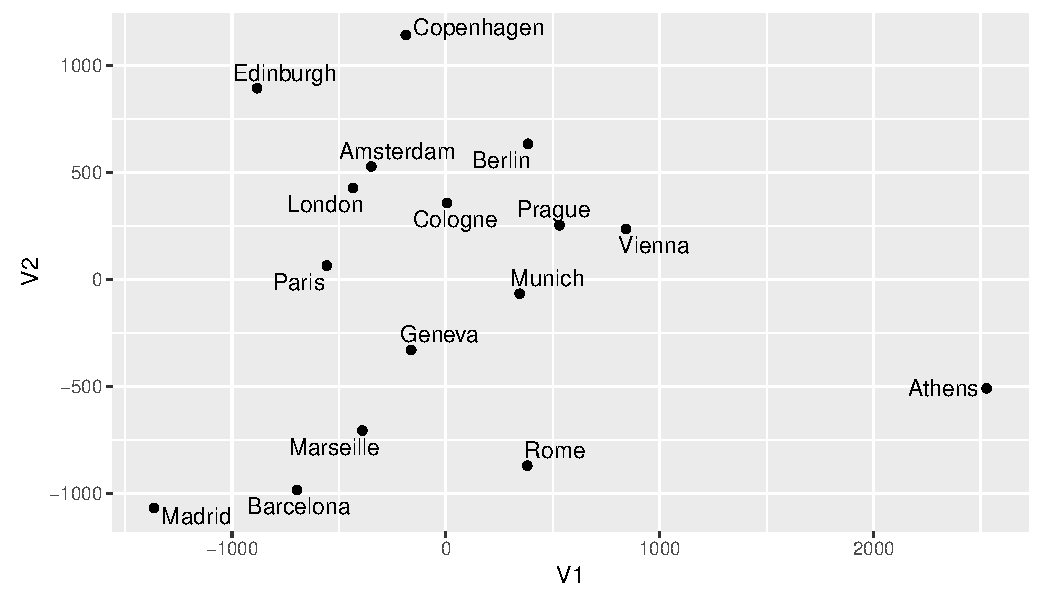
\includegraphics[width=\maxwidth]{figure/unnamed-chunk-9-1} 

\end{knitrout}
  
\end{frame}

\begin{frame}[fragile]{Comments}
  
  \begin{itemize}
  \item Tree shows how languages combined into clusters.
  \item First (bottom), Spanish, French, Italian joined into one
    cluster, Norwegian and Danish into another.
  \item Later, English joined to Norse languages, Polish to Romance group.
  \item Then German, Dutch make a Germanic group.
  \item Finally, Hungarian and Finnish joined to each other and
    everything else.
  \end{itemize}
  
\end{frame}

\begin{frame}[fragile]{Clustering process}

  \begin{minipage}[t]{0.45\linewidth}


    
{\small    
\begin{knitrout}
\definecolor{shadecolor}{rgb}{0.969, 0.969, 0.969}\color{fgcolor}\begin{kframe}
\begin{alltt}
\hlstd{d.hc}\hlopt{$}\hlstd{labels}
\end{alltt}
\begin{verbatim}
##  [1] "en" "no" "dk" "nl"
##  [5] "de" "fr" "es" "it"
##  [9] "pl" "hu" "fi"
\end{verbatim}
\begin{alltt}
\hlstd{d.hc}\hlopt{$}\hlstd{merge}
\end{alltt}
\begin{verbatim}
##       [,1] [,2]
##  [1,]   -2   -3
##  [2,]   -6   -8
##  [3,]   -7    2
##  [4,]   -1    1
##  [5,]   -9    3
##  [6,]   -5    4
##  [7,]   -4    6
##  [8,]    5    7
##  [9,]  -10    8
## [10,]  -11    9
\end{verbatim}
\end{kframe}
\end{knitrout}
}
  \end{minipage}
  \begin{minipage}[t]{0.5\linewidth}
    \vspace{0.5in}
    \begin{itemize}
    \item Lines of \texttt{merge} show what was combined
    \item First, languages 2 and 3 (\texttt{no} and \texttt{dk})
    \item Then languages 6 and 8 (\texttt{fr} and \texttt{it})
    \item Then \#7 combined with cluster formed at step 2 (\texttt{es}
      joined to \texttt{fr} and \texttt{it}.
    \item Then \texttt{en} joined to \texttt{no} and \texttt{dk} \ldots
    \item Finally \texttt{fi} joined to all others.
    \end{itemize}
  \end{minipage}

\end{frame}

\begin{frame}[fragile]{Complete linkage}
  
\begin{knitrout}
\definecolor{shadecolor}{rgb}{0.969, 0.969, 0.969}\color{fgcolor}\begin{kframe}
\begin{alltt}
\hlstd{d.hc}\hlkwb{=}\hlkwd{hclust}\hlstd{(d,}\hlkwc{method}\hlstd{=}\hlstr{"complete"}\hlstd{)}
\hlkwd{plot}\hlstd{(d.hc)}
\end{alltt}
\end{kframe}
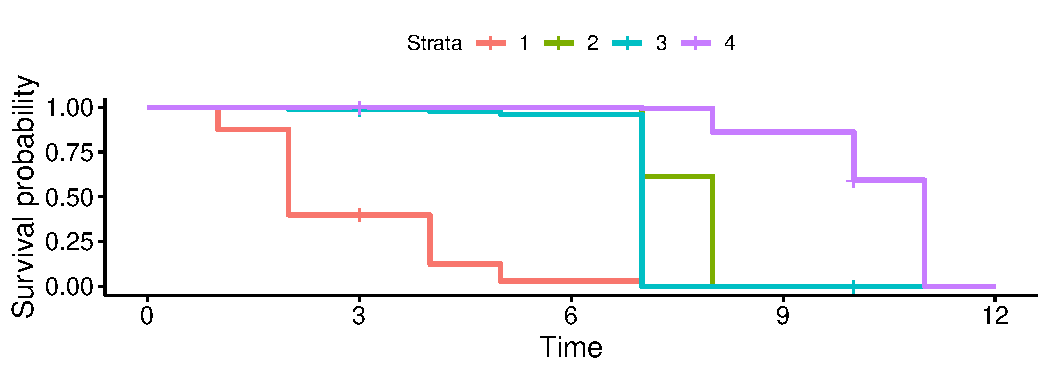
\includegraphics[width=\maxwidth]{figure/unnamed-chunk-12-1} 

\end{knitrout}
  
\end{frame}

\begin{frame}[fragile]{Ward}
  
\begin{knitrout}
\definecolor{shadecolor}{rgb}{0.969, 0.969, 0.969}\color{fgcolor}\begin{kframe}
\begin{alltt}
\hlstd{d.hc}\hlkwb{=}\hlkwd{hclust}\hlstd{(d,}\hlkwc{method}\hlstd{=}\hlstr{"ward.D"}\hlstd{)}
\hlkwd{plot}\hlstd{(d.hc)}
\end{alltt}
\end{kframe}
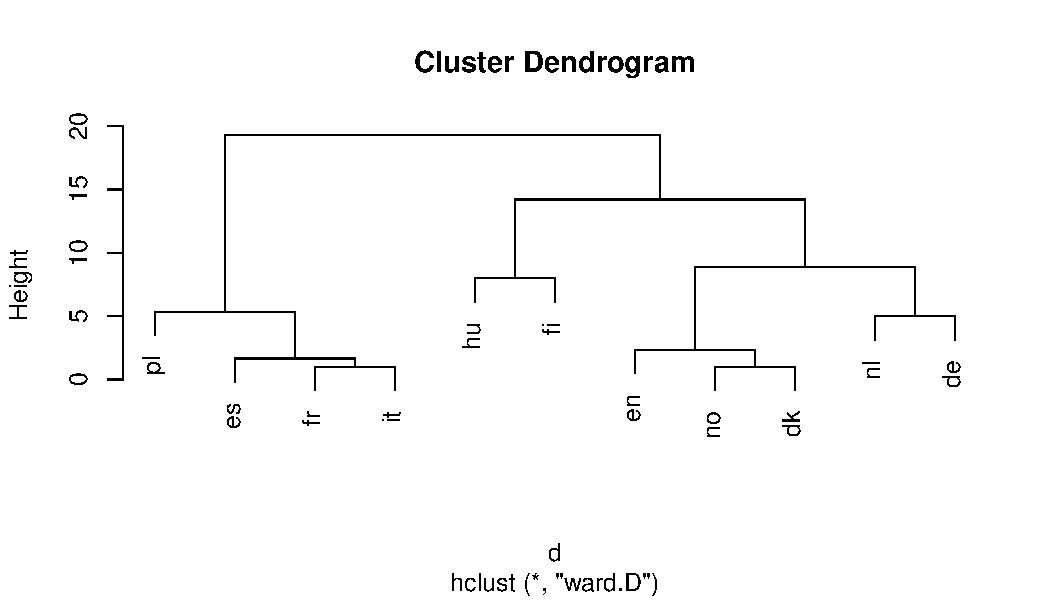
\includegraphics[width=\maxwidth]{figure/wardo-1} 

\end{knitrout}
  
\end{frame}

\begin{frame}[fragile]{Chopping the tree}

  \begin{itemize}
  \item Three clusters (from Ward) looks good:
\begin{knitrout}
\definecolor{shadecolor}{rgb}{0.969, 0.969, 0.969}\color{fgcolor}\begin{kframe}
\begin{alltt}
\hlkwd{cutree}\hlstd{(d.hc,}\hlnum{3}\hlstd{)}
\end{alltt}
\begin{verbatim}
## en no dk nl de fr es it 
##  1  1  1  1  1  2  2  2 
## pl hu fi 
##  2  3  3
\end{verbatim}
\end{kframe}
\end{knitrout}
  \end{itemize}
  
\end{frame}

\begin{frame}[fragile]{Drawing those clusters on the tree}
  
\begin{knitrout}
\definecolor{shadecolor}{rgb}{0.969, 0.969, 0.969}\color{fgcolor}\begin{kframe}
\begin{alltt}
\hlkwd{plot}\hlstd{(d.hc)}
\hlkwd{rect.hclust}\hlstd{(d.hc,}\hlnum{3}\hlstd{)}
\end{alltt}
\end{kframe}
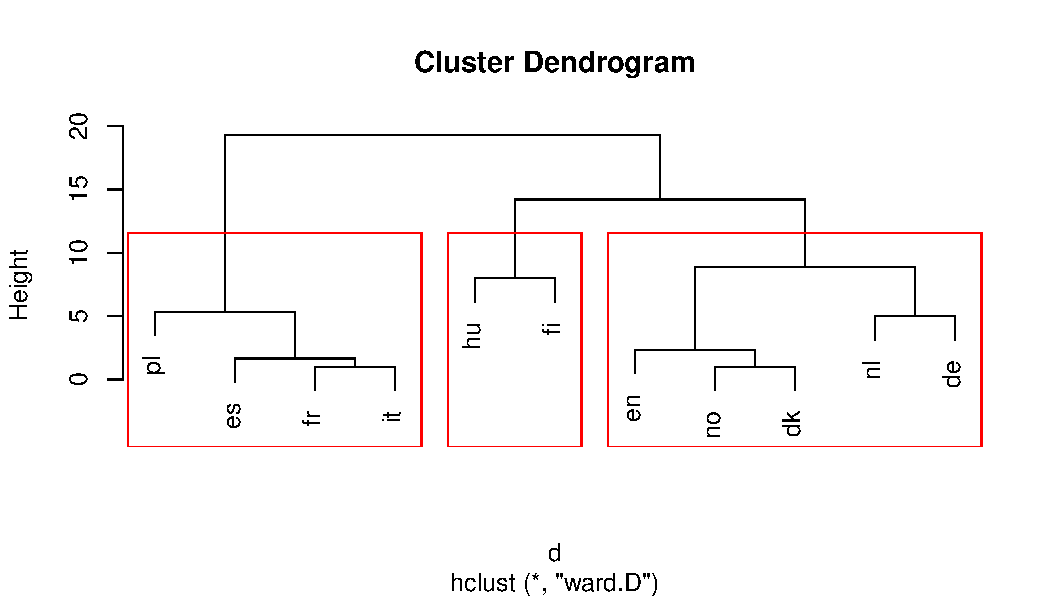
\includegraphics[width=\maxwidth]{figure/asfsagd-1} 

\end{knitrout}
  
\end{frame}

\begin{frame}[fragile]{Comparing single-linkage and Ward}

  \begin{itemize}
  \item In Ward, Dutch and German get joined earlier (before joining to Germanic cluster).
  \item Also Hungarian and Finnish get combined earlier.
  \end{itemize}
  
\end{frame}


\begin{frame}[fragile]{Making those dissimilarities}

Original data (part):




{\footnotesize
\begin{knitrout}
\definecolor{shadecolor}{rgb}{0.969, 0.969, 0.969}\color{fgcolor}\begin{kframe}
\begin{alltt}
\hlstd{lang}\hlkwb{=}\hlkwd{read.table}\hlstd{(}\hlstr{"one-ten.txt"}\hlstd{,}\hlkwc{header}\hlstd{=T,}\hlkwc{as.is}\hlstd{=}\hlnum{1}\hlopt{:}\hlnum{11}\hlstd{)}
\hlstd{lang} \hlopt \hlstd{dplyr}\hlopt{::}\hlkwd{select}\hlstd{(en}\hlopt{:}\hlstd{es)}
\end{alltt}
\begin{verbatim}
##       en   no   dk    nl     de     fr     es
## 1    one   en   en   een   eins     un    uno
## 2    two   to   to  twee   zwei   deux    dos
## 3  three  tre  tre  drie   drei  trois   tres
## 4   four fire fire  vier   vier quatre cuatro
## 5   five  fem  fem  vijf   funf   cinq  cinco
## 6    six seks seks   zes  sechs    six   seis
## 7  seven  sju  syv zeven sieben   sept  siete
## 8  eight atte otte  acht   acht   huit   ocho
## 9   nine   ni   ni negen   neun   neuf  nueve
## 10   ten   ti   ti  tien   zehn    dix   diez
\end{verbatim}
\end{kframe}
\end{knitrout}
}
  
\end{frame}

\begin{frame}[fragile]{Substrings}
  
Want to pull off the first character of those number names.




\begin{knitrout}
\definecolor{shadecolor}{rgb}{0.969, 0.969, 0.969}\color{fgcolor}\begin{kframe}
\begin{alltt}
\hlstd{v}\hlkwb{=}\hlkwd{c}\hlstd{(}\hlstr{"alpha"}\hlstd{,}\hlstr{"beta"}\hlstd{,}\hlstr{"gamma"}\hlstd{)}
\hlkwd{substr}\hlstd{(v,}\hlnum{1}\hlstd{,}\hlnum{2}\hlstd{)}
\end{alltt}
\begin{verbatim}
## [1] "al" "be" "ga"
\end{verbatim}
\begin{alltt}
\hlkwd{substr}\hlstd{(v,}\hlnum{3}\hlstd{,}\hlnum{3}\hlstd{)}
\end{alltt}
\begin{verbatim}
## [1] "p" "t" "m"
\end{verbatim}
\begin{alltt}
\hlstd{lang}\hlopt{$}\hlstd{en}
\end{alltt}
\begin{verbatim}
##  [1] "one"   "two"   "three" "four"  "five" 
##  [6] "six"   "seven" "eight" "nine"  "ten"
\end{verbatim}
\begin{alltt}
\hlkwd{substr}\hlstd{(lang}\hlopt{$}\hlstd{en,}\hlnum{1}\hlstd{,}\hlnum{1}\hlstd{)}
\end{alltt}
\begin{verbatim}
##  [1] "o" "t" "t" "f" "f" "s" "s" "e" "n" "t"
\end{verbatim}
\end{kframe}
\end{knitrout}

\begin{itemize}
\item 
\texttt{substr(s,i,j)} takes characters in \texttt{s} and extracts characters
from \texttt{i}th to \texttt{j}th inclusive. 
\item If \texttt{s} is vector, does it for all things in vector.
\end{itemize}
  
\end{frame}

\begin{frame}[fragile]{Array of first letters}

\begin{knitrout}\small
\definecolor{shadecolor}{rgb}{0.969, 0.969, 0.969}\color{fgcolor}\begin{kframe}
\begin{alltt}
\hlstd{lang.init}\hlkwb{=}\hlkwd{apply}\hlstd{(lang,}\hlnum{2}\hlstd{,substr,}\hlnum{1}\hlstd{,}\hlnum{1}\hlstd{)}
\hlstd{lang.init}
\end{alltt}
\begin{verbatim}
##       en  no  dk  nl  de  fr  es  it  pl  hu  fi 
##  [1,] "o" "e" "e" "e" "e" "u" "u" "u" "j" "e" "y"
##  [2,] "t" "t" "t" "t" "z" "d" "d" "d" "d" "k" "k"
##  [3,] "t" "t" "t" "d" "d" "t" "t" "t" "t" "h" "k"
##  [4,] "f" "f" "f" "v" "v" "q" "c" "q" "c" "n" "n"
##  [5,] "f" "f" "f" "v" "f" "c" "c" "c" "p" "o" "v"
##  [6,] "s" "s" "s" "z" "s" "s" "s" "s" "s" "h" "k"
##  [7,] "s" "s" "s" "z" "s" "s" "s" "s" "s" "h" "s"
##  [8,] "e" "a" "o" "a" "a" "h" "o" "o" "o" "n" "k"
##  [9,] "n" "n" "n" "n" "n" "n" "n" "n" "d" "k" "y"
## [10,] "t" "t" "t" "t" "z" "d" "d" "d" "d" "t" "k"
\end{verbatim}
\end{kframe}
\end{knitrout}

In \texttt{apply}: matrix, dimension to apply function to (columns, 2),
function to apply (\texttt{substr}), first and last char of substring.
  
\end{frame}

\begin{frame}[fragile]{Dealing with R \texttt{matrix}}
  
  \begin{itemize}
  \item What kind of thing is \texttt{lang.init}?
    
\begin{knitrout}
\definecolor{shadecolor}{rgb}{0.969, 0.969, 0.969}\color{fgcolor}\begin{kframe}
\begin{alltt}
\hlkwd{class}\hlstd{(lang.init)}
\end{alltt}
\begin{verbatim}
## [1] "matrix"
\end{verbatim}
\end{kframe}
\end{knitrout}

\item Matrices are like data frames, but:
  \begin{itemize}
  \item all their columns have to be the same type of thing, here text
  \item have to refer to columns by \emph{number} not name.
  \end{itemize}
  
\item Get hold of things like this:
  
\begin{knitrout}\footnotesize
\definecolor{shadecolor}{rgb}{0.969, 0.969, 0.969}\color{fgcolor}\begin{kframe}
\begin{alltt}
\hlstd{lang.init[}\hlnum{6}\hlstd{,}\hlnum{4}\hlstd{]}
\end{alltt}
\begin{verbatim}
##  nl 
## "z"
\end{verbatim}
\begin{alltt}
\hlstd{lang.init[}\hlnum{6}\hlstd{,]} \hlcom{# row 6, words for "six"}
\end{alltt}
\begin{verbatim}
##  en  no  dk  nl  de  fr  es  it  pl  hu  fi 
## "s" "s" "s" "z" "s" "s" "s" "s" "s" "h" "k"
\end{verbatim}
\begin{alltt}
\hlstd{lang.init[,}\hlnum{4}\hlstd{]} \hlcom{# column 4, Dutch}
\end{alltt}
\begin{verbatim}
##  [1] "e" "t" "d" "v" "v" "z" "z" "a" "n" "t"
\end{verbatim}
\end{kframe}
\end{knitrout}
  
  \end{itemize}
  
\end{frame}

\begin{frame}[fragile]{Comparing first letters}

Idea, with English (column 1) and Norwegian (column 2):




\begin{knitrout}\footnotesize
\definecolor{shadecolor}{rgb}{0.969, 0.969, 0.969}\color{fgcolor}\begin{kframe}
\begin{alltt}
\hlkwd{rbind}\hlstd{(lang.init[,}\hlnum{1}\hlstd{],lang.init[,}\hlnum{2}\hlstd{])}
\end{alltt}
\begin{verbatim}
##      [,1] [,2] [,3] [,4] [,5] [,6] [,7] [,8] [,9] [,10]
## [1,] "o"  "t"  "t"  "f"  "f"  "s"  "s"  "e"  "n"  "t"  
## [2,] "e"  "t"  "t"  "f"  "f"  "s"  "s"  "a"  "n"  "t"
\end{verbatim}
\begin{alltt}
\hlstd{different}\hlkwb{=}\hlstd{(lang.init[,}\hlnum{1}\hlstd{]}\hlopt{!=}\hlstd{lang.init[,}\hlnum{2}\hlstd{])}
\hlstd{different}
\end{alltt}
\begin{verbatim}
##  [1]  TRUE FALSE FALSE FALSE FALSE FALSE FALSE  TRUE FALSE
## [10] FALSE
\end{verbatim}
\begin{alltt}
\hlkwd{sum}\hlstd{(different)}
\end{alltt}
\begin{verbatim}
## [1] 2
\end{verbatim}
\end{kframe}
\end{knitrout}

This does English and Norwegian. For others, change 1 and 2 to
\texttt{i} and \texttt{j}, make into function.
  
\end{frame}

\begin{frame}[fragile]{Language-comparing function}
  
  Input is numbers of two languages to compare:
  
\begin{knitrout}
\definecolor{shadecolor}{rgb}{0.969, 0.969, 0.969}\color{fgcolor}\begin{kframe}
\begin{alltt}
\hlstd{count.diff}\hlkwb{=}\hlkwa{function}\hlstd{(}\hlkwc{i}\hlstd{,}\hlkwc{j}\hlstd{)}
  \hlstd{\{}
    \hlstd{diff}\hlkwb{=}\hlstd{(lang.init[,i]}\hlopt{!=}\hlstd{lang.init[,j])}
    \hlkwd{sum}\hlstd{(diff)}
  \hlstd{\}}

\hlkwd{count.diff}\hlstd{(}\hlnum{1}\hlstd{,}\hlnum{2}\hlstd{)}
\end{alltt}
\begin{verbatim}
## [1] 2
\end{verbatim}
\begin{alltt}
\hlkwd{count.diff}\hlstd{(}\hlnum{9}\hlstd{,}\hlnum{10}\hlstd{)}
\end{alltt}
\begin{verbatim}
## [1] 10
\end{verbatim}
\end{kframe}
\end{knitrout}

English and Norwegian have 2 different, Polish and Hungarian all 10.
  
\end{frame}

\begin{frame}[fragile]{A loop to compare all pairs}
  
    
\begin{knitrout}
\definecolor{shadecolor}{rgb}{0.969, 0.969, 0.969}\color{fgcolor}\begin{kframe}
\begin{alltt}
\hlstd{dd}\hlkwb{=}\hlkwd{matrix}\hlstd{(}\hlnum{0}\hlstd{,}\hlnum{11}\hlstd{,}\hlnum{11}\hlstd{)}
\hlkwa{for} \hlstd{(i} \hlkwa{in} \hlnum{1}\hlopt{:}\hlnum{11}\hlstd{)}
\hlstd{\{}
  \hlkwa{for} \hlstd{(j} \hlkwa{in} \hlnum{1}\hlopt{:}\hlnum{11}\hlstd{)}
    \hlstd{\{}
      \hlstd{dd[i,j]}\hlkwb{=}\hlkwd{count.diff}\hlstd{(i,j)}
    \hlstd{\}}
\hlstd{\}}
\end{alltt}
\end{kframe}
\end{knitrout}

\begin{itemize}
\item First line makes an $11\times 11$ matrix of 0s (there are 11
  languages).
\item Then loop through each \emph{pair} of languages, see how many
  number names start with a different letter, and store in right place.
\end{itemize}
\end{frame}

\begin{frame}[fragile]{The results}


  
  
{\footnotesize  
\begin{knitrout}
\definecolor{shadecolor}{rgb}{0.969, 0.969, 0.969}\color{fgcolor}\begin{kframe}
\begin{alltt}
\hlstd{dd}
\end{alltt}
\begin{verbatim}
##       [,1] [,2] [,3] [,4] [,5] [,6] [,7] [,8] [,9] [,10] [,11]
##  [1,]    0    2    2    7    6    6    6    6    7     9     9
##  [2,]    2    0    1    5    4    6    6    6    7     8     9
##  [3,]    2    1    0    6    5    6    5    5    6     8     9
##  [4,]    7    5    6    0    5    9    9    9   10     8     9
##  [5,]    6    4    5    5    0    7    7    7    8     9     9
##  [6,]    6    6    6    9    7    0    2    1    5    10     9
##  [7,]    6    6    5    9    7    2    0    1    3    10     9
##  [8,]    6    6    5    9    7    1    1    0    4    10     9
##  [9,]    7    7    6   10    8    5    3    4    0    10     9
## [10,]    9    8    8    8    9   10   10   10   10     0     8
## [11,]    9    9    9    9    9    9    9    9    9     8     0
\end{verbatim}
\end{kframe}
\end{knitrout}
}

The same as \texttt{number.d} earlier.
  
\end{frame}


\begin{frame}[fragile]{Another example}

Birth, death and infant mortality rates for 97 countries (variables not dissimilarities):

{\scriptsize
\begin{verbatim}
   24.7  5.7  30.8 Albania             12.5 11.9  14.4 Bulgaria
   13.4 11.7  11.3 Czechoslovakia      12   12.4   7.6 Former_E._Germany
   11.6 13.4  14.8 Hungary             14.3 10.2    16 Poland
   13.6 10.7  26.9 Romania               14    9  20.2 Yugoslavia
   17.7   10    23 USSR                15.2  9.5  13.1 Byelorussia_SSR
   13.4 11.6    13 Ukrainian_SSR       20.7  8.4  25.7 Argentina
   46.6   18   111 Bolivia             28.6  7.9    63 Brazil
   23.4  5.8  17.1 Chile               27.4  6.1    40 Columbia
   32.9  7.4    63 Ecuador             28.3  7.3    56 Guyana
...
\end{verbatim}
}

\begin{itemize}
\item Want to find groups of similar countries (and how many groups, which countries in each group).
\item Tree would be unwieldy with 97 countries.
\item More automatic way of finding given number of clusters?
\end{itemize}
  
\end{frame}

\begin{frame}[fragile]{Pre-processing}

  \begin{itemize}
  \item Country names will get read in as factor, but want as text (for
    later), hence \texttt{stringsAsFactors}.
  \end{itemize}
  
{\scriptsize
\begin{knitrout}
\definecolor{shadecolor}{rgb}{0.969, 0.969, 0.969}\color{fgcolor}\begin{kframe}
\begin{alltt}
\hlstd{vital}\hlkwb{=}\hlkwd{read.table}\hlstd{(}\hlstr{"birthrate.txt"}\hlstd{,}\hlkwc{header}\hlstd{=T,}\hlkwc{stringsAsFactors}\hlstd{=F)}
\hlkwd{str}\hlstd{(vital)}
\end{alltt}
\begin{verbatim}
## 'data.frame':	97 obs. of  4 variables:
##  $ birth  : num  24.7 13.4 11.6 13.6 17.7 13.4 46.6 23.4 32.9 34.8 ...
##  $ death  : num  5.7 11.7 13.4 10.7 10 11.6 18 5.8 7.4 6.6 ...
##  $ infant : num  30.8 11.3 14.8 26.9 23 13 111 17.1 63 42 ...
##  $ country: chr  "Albania" "Czechoslovakia" "Hungary" "Romania" ...
\end{verbatim}
\end{kframe}
\end{knitrout}
}
\end{frame}

\begin{frame}[fragile]{Standardizing}


\begin{itemize}
\item Infant mortality rate numbers bigger than others, consequence of
  measurement scale (arbitrary).
\item Standardize (numerical) columns of data frame to have mean 0, SD
  1, done by \texttt{scale}.
\item Create data frame with column of abbreviated names (for later).
  \end{itemize}

\begin{knitrout}\footnotesize
\definecolor{shadecolor}{rgb}{0.969, 0.969, 0.969}\color{fgcolor}\begin{kframe}
\begin{alltt}
\hlstd{vital.s}\hlkwb{=}\hlkwd{with}\hlstd{(vital,}\hlkwd{data.frame}\hlstd{(}\hlkwc{birth}\hlstd{=}\hlkwd{scale}\hlstd{(birth),}
                     \hlkwc{death}\hlstd{=}\hlkwd{scale}\hlstd{(death),} \hlkwc{infant}\hlstd{=}\hlkwd{scale}\hlstd{(infant),}
                     \hlkwc{country}\hlstd{=country,} \hlkwc{stringsAsFactors}\hlstd{=F))}
\hlkwd{head}\hlstd{(vital.s)}
\end{alltt}
\begin{verbatim}
##        birth       death     infant        country
## 1 -0.3343913 -1.10512932 -0.5240199        Albania
## 2 -1.1685431  0.18588887 -0.9480013 Czechoslovakia
## 3 -1.3014168  0.55167736 -0.8719021        Hungary
## 4 -1.1537793 -0.02928083 -0.6088162        Romania
## 5 -0.8511225 -0.17989961 -0.6936125           USSR
## 6 -1.1685431  0.16437190 -0.9110388  Ukrainian_SSR
\end{verbatim}
\end{kframe}
\end{knitrout}
  
\end{frame}

\begin{frame}[fragile]{Three clusters}
  
  Pretending we know 3 clusters is good:



{\small
\begin{knitrout}
\definecolor{shadecolor}{rgb}{0.969, 0.969, 0.969}\color{fgcolor}\begin{kframe}
\begin{alltt}
\hlstd{vital.km3}\hlkwb{=}\hlkwd{kmeans}\hlstd{(vital.s[,}\hlnum{1}\hlopt{:}\hlnum{3}\hlstd{],}\hlnum{3}\hlstd{)}
\hlkwd{names}\hlstd{(vital.km3)}
\end{alltt}
\begin{verbatim}
## [1] "cluster"      "centers"      "totss"        "withinss"    
## [5] "tot.withinss" "betweenss"    "size"         "iter"        
## [9] "ifault"
\end{verbatim}
\end{kframe}
\end{knitrout}
  }
  
  A lot of output, so look at these individually.
  
\end{frame}


\begin{frame}[fragile]{What's in the output?}
  
  \begin{itemize}
  \item Cluster sizes:
    

\begin{knitrout}
\definecolor{shadecolor}{rgb}{0.969, 0.969, 0.969}\color{fgcolor}\begin{kframe}
\begin{alltt}
\hlstd{vital.km3}\hlopt{$}\hlstd{size}
\end{alltt}
\begin{verbatim}
## [1] 29 44 24
\end{verbatim}
\end{kframe}
\end{knitrout}

\item Cluster centres:
  
\begin{knitrout}
\definecolor{shadecolor}{rgb}{0.969, 0.969, 0.969}\color{fgcolor}\begin{kframe}
\begin{alltt}
\hlstd{vital.km3}\hlopt{$}\hlstd{centers}
\end{alltt}
\begin{verbatim}
##        birth      death     infant
## 1  0.4737967 -0.4878149  0.2466440
## 2 -0.9593341 -0.4322350 -0.8904328
## 3  1.1862748  1.3818738  1.3344318
\end{verbatim}
\end{kframe}
\end{knitrout}

\item Cluster 2 has lower than average rates on everything; cluster 3
  has much higher than average.
    
  \end{itemize}
  
\end{frame}

\begin{frame}[fragile]{Cluster sums of squares and membership}
  
\begin{knitrout}
\definecolor{shadecolor}{rgb}{0.969, 0.969, 0.969}\color{fgcolor}\begin{kframe}
\begin{alltt}
\hlstd{vital.km3}\hlopt{$}\hlstd{withinss}
\end{alltt}
\begin{verbatim}
## [1] 14.96356 25.13922 26.78049
\end{verbatim}
\end{kframe}
\end{knitrout}

Cluster 1 compact relative to others (countries in cluster 1  more similar).

\begin{knitrout}
\definecolor{shadecolor}{rgb}{0.969, 0.969, 0.969}\color{fgcolor}\begin{kframe}
\begin{alltt}
\hlstd{vital.km3}\hlopt{$}\hlstd{cluster}
\end{alltt}
\begin{verbatim}
##  [1] 2 2 2 2 2 2 3 2 1 1 2 3 2 2 2 2 2 2 2 2 2 3 1
## [24] 2 2 1 1 3 2 1 2 1 1 2 2 1 1 1 3 3 1 1 3 3 1 3
## [47] 3 3 1 2 2 2 2 2 2 1 1 1 1 2 2 2 2 2 2 2 2 2 2
## [70] 2 2 1 1 1 1 2 3 2 1 1 3 1 2 1 3 3 3 3 1 3 3 3
## [93] 3 3 1 3 3
\end{verbatim}
\begin{alltt}
\hlstd{vital.s}\hlopt{$}\hlstd{cluster}\hlkwb{=}\hlstd{vital.km3}\hlopt{$}\hlstd{cluster}
\end{alltt}
\end{kframe}
\end{knitrout}

Next, which countries in which cluster?

  
\end{frame}


\begin{frame}[fragile]{Cluster membership: cluster 2}


\begin{knitrout}\footnotesize
\definecolor{shadecolor}{rgb}{0.969, 0.969, 0.969}\color{fgcolor}\begin{kframe}
\begin{alltt}
\hlkwd{with}\hlstd{(vital.s,country[cluster}\hlopt{==}\hlnum{2}\hlstd{])}
\end{alltt}
\begin{verbatim}
##  [1] "Albania"              "Czechoslovakia"       "Hungary"             
##  [4] "Romania"              "USSR"                 "Ukrainian_SSR"       
##  [7] "Chile"                "Uruguay"              "Finland"             
## [10] "France"               "Greece"               "Italy"               
## [13] "Norway"               "Spain"                "Switzerland"         
## [16] "Austria"              "Canada"               "Israel"              
## [19] "Kuwait"               "China"                "Korea"               
## [22] "Singapore"            "Thailand"             "Bulgaria"            
## [25] "Former_E._Germany"    "Poland"               "Yugoslavia"          
## [28] "Byelorussia_SSR"      "Argentina"            "Venezuela"           
## [31] "Belgium"              "Denmark"              "Germany"             
## [34] "Ireland"              "Netherlands"          "Portugal"            
## [37] "Sweden"               "U.K."                 "Japan"               
## [40] "U.S.A."               "Bahrain"              "United_Arab_Emirates"
## [43] "Hong_Kong"            "Sri_Lanka"
\end{verbatim}
\end{kframe}
\end{knitrout}

\end{frame}

\begin{frame}[fragile]{Cluster 3}
\begin{knitrout}\footnotesize
\definecolor{shadecolor}{rgb}{0.969, 0.969, 0.969}\color{fgcolor}\begin{kframe}
\begin{alltt}
\hlkwd{with}\hlstd{(vital.s,country[cluster}\hlopt{==}\hlnum{3}\hlstd{])}
\end{alltt}
\begin{verbatim}
##  [1] "Bolivia"      "Mexico"       "Afghanistan" 
##  [4] "Bangladesh"   "Gabon"        "Ghana"       
##  [7] "Namibia"      "Sierra_Leone" "Swaziland"   
## [10] "Uganda"       "Zaire"        "Cambodia"    
## [13] "Nepal"        "Angola"       "Congo"       
## [16] "Ethiopia"     "Gambia"       "Malawi"      
## [19] "Mozambique"   "Nigeria"      "Somalia"     
## [22] "Sudan"        "Tanzania"     "Zambia"
\end{verbatim}
\end{kframe}
\end{knitrout}
\end{frame}

\begin{frame}[fragile]{Cluster 1}

\begin{knitrout}\footnotesize
\definecolor{shadecolor}{rgb}{0.969, 0.969, 0.969}\color{fgcolor}\begin{kframe}
\begin{alltt}
\hlkwd{with}\hlstd{(vital.s,country[cluster}\hlopt{==}\hlnum{1}\hlstd{])}
\end{alltt}
\begin{verbatim}
##  [1] "Ecuador"      "Paraguay"     "Iran"        
##  [4] "Oman"         "Turkey"       "India"       
##  [7] "Mongolia"     "Pakistan"     "Algeria"     
## [10] "Botswana"     "Egypt"        "Libya"       
## [13] "Morocco"      "South_Africa" "Zimbabwe"    
## [16] "Brazil"       "Columbia"     "Guyana"      
## [19] "Peru"         "Iraq"         "Jordan"      
## [22] "Lebanon"      "Saudi_Arabia" "Indonesia"   
## [25] "Malaysia"     "Philippines"  "Vietnam"     
## [28] "Kenya"        "Tunisia"
\end{verbatim}
\end{kframe}
\end{knitrout}
\end{frame}

\begin{frame}[fragile]{Problem!}
  
  \begin{itemize}
  \item \texttt{kmeans} uses randomization. So result of one run might
    be different from another run.
  \item Example: just run again on 3 clusters, \texttt{table} of results:

    
\begin{knitrout}
\definecolor{shadecolor}{rgb}{0.969, 0.969, 0.969}\color{fgcolor}\begin{kframe}
\begin{alltt}
\hlstd{vital.km3a}\hlkwb{=}\hlkwd{kmeans}\hlstd{(vital.s[}\hlnum{1}\hlopt{:}\hlnum{3}\hlstd{],}\hlnum{3}\hlstd{)}
\hlkwd{table}\hlstd{(}\hlkwc{first}\hlstd{=vital.km3}\hlopt{$}\hlstd{cluster,}
      \hlkwc{second}\hlstd{=vital.km3a}\hlopt{$}\hlstd{cluster)}
\end{alltt}
\begin{verbatim}
##      second
## first  1  2  3
##     1  1  0 28
##     2  0 40  4
##     3 24  0  0
\end{verbatim}
\end{kframe}
\end{knitrout}
\item Solution: \texttt{nstart} option on \texttt{kmeans} runs that
  many times, takes best. Should be same every time:
\begin{knitrout}
\definecolor{shadecolor}{rgb}{0.969, 0.969, 0.969}\color{fgcolor}\begin{kframe}
\begin{alltt}
\hlstd{vital.km3b}\hlkwb{=}\hlkwd{kmeans}\hlstd{(vital.s,}\hlnum{3}\hlstd{,}\hlkwc{nstart}\hlstd{=}\hlnum{20}\hlstd{)}
\end{alltt}
\end{kframe}
\end{knitrout}
    
    
  \end{itemize}
  
\end{frame}

\begin{frame}[fragile]{How many clusters?}
  
  \begin{itemize}
  \item Three was just a guess.
  \item Idea: try a whole bunch of \#clusters (say 2--20), obtain measure of
    goodness of fit for each, make plot.
  \item Appropriate measure is \texttt{tot.withinss}.
  \item Use loop to run \texttt{kmeans} for each \#clusters, keep
    track of \texttt{tot.withinss}.
  \end{itemize}
  
\end{frame}

\begin{frame}[fragile]{Making this happen}
  
\begin{knitrout}
\definecolor{shadecolor}{rgb}{0.969, 0.969, 0.969}\color{fgcolor}\begin{kframe}
\begin{alltt}
\hlstd{clus}\hlkwb{=}\hlnum{2}\hlopt{:}\hlnum{20}
\hlstd{wss}\hlkwb{=}\hlkwd{numeric}\hlstd{(}\hlnum{0}\hlstd{)}
\hlkwa{for} \hlstd{(i} \hlkwa{in} \hlstd{clus)}
\hlstd{\{}
  \hlstd{wss[i]}\hlkwb{=}\hlkwd{kmeans}\hlstd{(vital.s[}\hlnum{1}\hlopt{:}\hlnum{3}\hlstd{],i,}\hlkwc{nstart}\hlstd{=}\hlnum{20}\hlstd{)}\hlopt{$}\hlstd{tot.withinss}
\hlstd{\}}
\hlstd{wss}
\end{alltt}
\begin{verbatim}
##  [1]         NA 117.375682  66.883275  51.403362
##  [5]  37.513143  28.659864  24.714303  22.296955
##  [9]  19.632431  17.472883  16.207393  14.956056
## [13]  13.242480  12.127228  11.741309  10.676895
## [17]   9.526443   9.058126   8.597169   7.577362
\end{verbatim}
\end{kframe}
\end{knitrout}
  
\end{frame}

\begin{frame}[fragile]{A more R way to do it}
  
  \begin{itemize}
  \item Define a function whose input is the number of clusters and
    whose output is the total within-cluster sum of squares:
    
\begin{knitrout}
\definecolor{shadecolor}{rgb}{0.969, 0.969, 0.969}\color{fgcolor}\begin{kframe}
\begin{alltt}
\hlstd{wssf}\hlkwb{=}\hlkwa{function}\hlstd{(}\hlkwc{nclust}\hlstd{) \{}
  \hlkwd{kmeans}\hlstd{(vital.s[}\hlnum{1}\hlopt{:}\hlnum{3}\hlstd{],nclust,}\hlkwc{nstart}\hlstd{=}\hlnum{20}\hlstd{)}\hlopt{$}\hlstd{tot.withinss}
\hlstd{\}}
\hlkwd{wssf}\hlstd{(}\hlnum{2}\hlstd{)}
\end{alltt}
\begin{verbatim}
## [1] 117.3757
\end{verbatim}
\end{kframe}
\end{knitrout}
%$ %$ %$ 

\item Feed that into \texttt{sapply} thus (``for each value of the
  first thing, run function that is second thing''):
  
\begin{knitrout}\small
\definecolor{shadecolor}{rgb}{0.969, 0.969, 0.969}\color{fgcolor}\begin{kframe}
\begin{alltt}
\hlstd{wss}\hlkwb{=}\hlkwd{sapply}\hlstd{(clus,wssf)}
\hlstd{wss}
\end{alltt}
\begin{verbatim}
##  [1] 117.375682  66.883275  51.403362  37.513143
##  [5]  28.659864  24.714303  22.016306  19.640729
##  [9]  17.472883  16.317851  15.140205  13.395265
## [13]  12.423674  11.168144  10.520674   9.830072
## [17]   9.372249   8.318697   7.298821
\end{verbatim}
\end{kframe}
\end{knitrout}

  \end{itemize}
  
\end{frame}

\begin{frame}[fragile]{Scree plot}

\begin{knitrout}
\definecolor{shadecolor}{rgb}{0.969, 0.969, 0.969}\color{fgcolor}\begin{kframe}
\begin{alltt}
\hlstd{d}\hlkwb{=}\hlkwd{data.frame}\hlstd{(clus,wss)}
\hlkwd{ggplot}\hlstd{(d,}\hlkwd{aes}\hlstd{(}\hlkwc{x}\hlstd{=clus,}\hlkwc{y}\hlstd{=wss))}\hlopt{+}\hlkwd{geom_point}\hlstd{()}\hlopt{+}\hlkwd{geom_line}\hlstd{()}
\end{alltt}
\end{kframe}
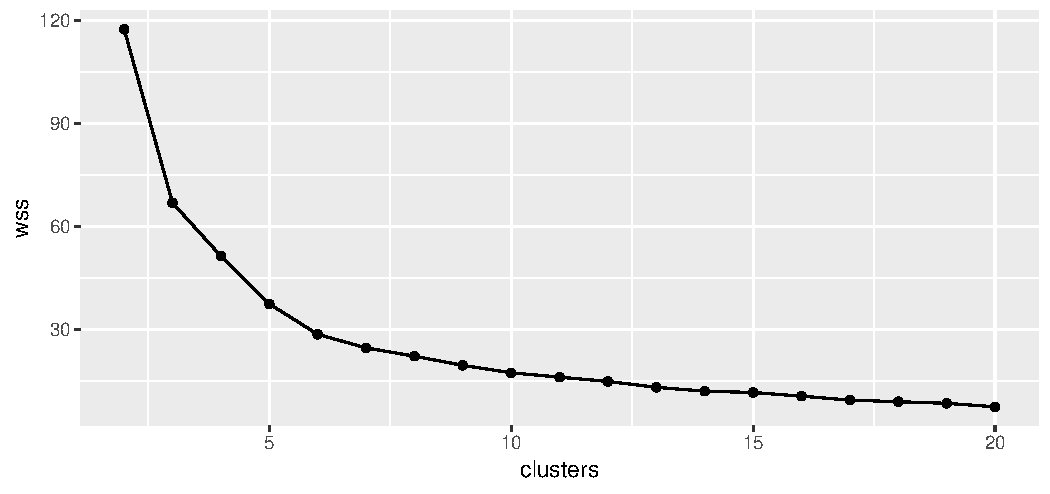
\includegraphics[width=\maxwidth]{figure/favalli-1} 

\end{knitrout}
  
\end{frame}

\begin{frame}[fragile]{Interpreting scree plot}
  
  \begin{itemize}
  \item Lower \texttt{wss} better.
  \item But lower for larger \#clusters, harder to explain.
  \item Compromise: low-ish \texttt{wss} and low-ish \#clusters.
  \item Look for ``elbow'' in plot.
  \item Idea: this is where \texttt{wss} decreases fast then slow.
  \item On our plot, small elbow at 6 clusters. Try this many clusters.
  \end{itemize}
  
\end{frame}

\begin{frame}[fragile]{Six clusters, using \texttt{nstart}}
  
\begin{knitrout}
\definecolor{shadecolor}{rgb}{0.969, 0.969, 0.969}\color{fgcolor}\begin{kframe}
\begin{alltt}
\hlstd{vital.km6}\hlkwb{=}\hlkwd{kmeans}\hlstd{(vital.s[}\hlnum{1}\hlopt{:}\hlnum{3}\hlstd{],}\hlnum{6}\hlstd{,}\hlkwc{nstart}\hlstd{=}\hlnum{20}\hlstd{)}
\hlstd{vital.km6}\hlopt{$}\hlstd{size}
\end{alltt}
\begin{verbatim}
## [1]  8 30 24 15 18  2
\end{verbatim}
\begin{alltt}
\hlstd{vital.km6}\hlopt{$}\hlstd{centers}
\end{alltt}
\begin{verbatim}
##        birth      death     infant
## 1  1.3043848  2.1896567  1.9470306
## 2 -1.1737104 -0.1856375 -0.9534370
## 3  0.4160993 -0.5169988  0.2648754
## 4 -0.4357690 -1.1438599 -0.7281108
## 5  1.2092406  0.7441347  1.0278003
## 6 -0.2199722  2.1116577 -0.4544435
\end{verbatim}
\begin{alltt}
\hlstd{vital.s}\hlopt{$}\hlstd{clus6}\hlkwb{=}\hlstd{vital.km6}\hlopt{$}\hlstd{cluster}
\end{alltt}
\end{kframe}
\end{knitrout}
  
\end{frame}

\begin{frame}[fragile]{Cluster 1}

    High on everything:

  
\begin{knitrout}
\definecolor{shadecolor}{rgb}{0.969, 0.969, 0.969}\color{fgcolor}\begin{kframe}
\begin{alltt}
\hlkwd{with}\hlstd{(vital.s,country[clus6}\hlopt{==}\hlnum{1}\hlstd{])}
\end{alltt}
\begin{verbatim}
## [1] "Afghanistan"  "Sierra_Leone" "Angola"      
## [4] "Ethiopia"     "Gambia"       "Malawi"      
## [7] "Mozambique"   "Somalia"
\end{verbatim}
\end{kframe}
\end{knitrout}
  
\end{frame}
\begin{frame}[fragile]{Cluster 2}

  Low on everything, though death rate close to average:
  
\begin{knitrout}\small
\definecolor{shadecolor}{rgb}{0.969, 0.969, 0.969}\color{fgcolor}\begin{kframe}
\begin{alltt}
\hlkwd{with}\hlstd{(vital.s,country[clus6}\hlopt{==}\hlnum{2}\hlstd{])}
\end{alltt}
\begin{verbatim}
##  [1] "Czechoslovakia"    "Hungary"           "Romania"          
##  [4] "USSR"              "Ukrainian_SSR"     "Uruguay"          
##  [7] "Finland"           "France"            "Greece"           
## [10] "Italy"             "Norway"            "Spain"            
## [13] "Switzerland"       "Austria"           "Canada"           
## [16] "Bulgaria"          "Former_E._Germany" "Poland"           
## [19] "Yugoslavia"        "Byelorussia_SSR"   "Belgium"          
## [22] "Denmark"           "Germany"           "Ireland"          
## [25] "Netherlands"       "Portugal"          "Sweden"           
## [28] "U.K."              "Japan"             "U.S.A."
\end{verbatim}
\end{kframe}
\end{knitrout}
  
\end{frame}
\begin{frame}[fragile]{Cluster 3}

  Below-average death rate, though other rates a little higher than average:

  
\begin{knitrout}
\definecolor{shadecolor}{rgb}{0.969, 0.969, 0.969}\color{fgcolor}\begin{kframe}
\begin{alltt}
\hlkwd{with}\hlstd{(vital.s,country[clus6}\hlopt{==}\hlnum{3}\hlstd{])}
\end{alltt}
\begin{verbatim}
##  [1] "Ecuador"      "Paraguay"     "Oman"        
##  [4] "Turkey"       "India"        "Mongolia"    
##  [7] "Pakistan"     "Algeria"      "Egypt"       
## [10] "Libya"        "Morocco"      "South_Africa"
## [13] "Zimbabwe"     "Brazil"       "Guyana"      
## [16] "Peru"         "Iraq"         "Jordan"      
## [19] "Lebanon"      "Saudi_Arabia" "Indonesia"   
## [22] "Philippines"  "Vietnam"      "Tunisia"
\end{verbatim}
\end{kframe}
\end{knitrout}
  
\end{frame}
\begin{frame}[fragile]{Cluster 4}

    Low on everything, especially death rate:

  
\begin{knitrout}
\definecolor{shadecolor}{rgb}{0.969, 0.969, 0.969}\color{fgcolor}\begin{kframe}
\begin{alltt}
\hlkwd{with}\hlstd{(vital.s,country[clus6}\hlopt{==}\hlnum{4}\hlstd{])}
\end{alltt}
\begin{verbatim}
##  [1] "Albania"              "Chile"               
##  [3] "Israel"               "Kuwait"              
##  [5] "China"                "Singapore"           
##  [7] "Thailand"             "Argentina"           
##  [9] "Columbia"             "Venezuela"           
## [11] "Bahrain"              "United_Arab_Emirates"
## [13] "Hong_Kong"            "Malaysia"            
## [15] "Sri_Lanka"
\end{verbatim}
\end{kframe}
\end{knitrout}
  
\end{frame}
\begin{frame}[fragile]{Cluster 5}

  Higher than average on everything, though not the highest:
  
\begin{knitrout}
\definecolor{shadecolor}{rgb}{0.969, 0.969, 0.969}\color{fgcolor}\begin{kframe}
\begin{alltt}
\hlkwd{with}\hlstd{(vital.s,country[clus6}\hlopt{==}\hlnum{5}\hlstd{])}
\end{alltt}
\begin{verbatim}
##  [1] "Bolivia"    "Iran"       "Bangladesh"
##  [4] "Botswana"   "Gabon"      "Ghana"     
##  [7] "Namibia"    "Swaziland"  "Uganda"    
## [10] "Zaire"      "Cambodia"   "Nepal"     
## [13] "Congo"      "Kenya"      "Nigeria"   
## [16] "Sudan"      "Tanzania"   "Zambia"
\end{verbatim}
\end{kframe}
\end{knitrout}
  
\end{frame}
\begin{frame}[fragile]{Cluster 6}

    Very high death rate, just below average on all else:

  
\begin{knitrout}
\definecolor{shadecolor}{rgb}{0.969, 0.969, 0.969}\color{fgcolor}\begin{kframe}
\begin{alltt}
\hlkwd{with}\hlstd{(vital.s,country[clus6}\hlopt{==}\hlnum{6}\hlstd{])}
\end{alltt}
\begin{verbatim}
## [1] "Mexico" "Korea"
\end{verbatim}
\end{kframe}
\end{knitrout}
  
\end{frame}

\begin{frame}[fragile]{Comparing our 3 and 6-cluster solutions}
  
\begin{knitrout}
\definecolor{shadecolor}{rgb}{0.969, 0.969, 0.969}\color{fgcolor}\begin{kframe}
\begin{alltt}
\hlkwd{table}\hlstd{(}\hlkwc{three}\hlstd{=vital.km3}\hlopt{$}\hlstd{cluster,}\hlkwc{six}\hlstd{=vital.km6}\hlopt{$}\hlstd{cluster)}
\end{alltt}
\begin{verbatim}
##      six
## three  1  2  3  4  5  6
##     1  0  0 24  2  3  0
##     2  0 30  0 13  0  1
##     3  8  0  0  0 15  1
\end{verbatim}
\end{kframe}
\end{knitrout}

Compared to 3-cluster solution:

\begin{itemize}
\item most of cluster 1 gone to cluster 3
\item cluster 2 split into clusters 2 and 4 (two types of ``richer'' countries)
\item cluster 3 split into clusters 1 and 5 (two types of ``poor''
  countries, divided by death rate).
\end{itemize}
  
\end{frame}


\begin{frame}[fragile]{Getting a picture from \texttt{kmeans}}
  
  \begin{itemize}
  \item Use multidimensional scaling (later)
  \item Use discriminant analysis on clusters found, treating them as
    ``known'' groups.
  \end{itemize}
  
\end{frame}


\begin{frame}[fragile]{MANOVA and discriminant analysis}
  
  \begin{itemize}
  \item Go back to 1st 3 columns of \texttt{vital.s} (variables,
    standardized), plus \texttt{cf} (cluster as factor).
    \texttt{clus} (6 clusters).
  \item First, do they actually differ by group? (MANOVA):
    {\small
\begin{knitrout}
\definecolor{shadecolor}{rgb}{0.969, 0.969, 0.969}\color{fgcolor}\begin{kframe}
\begin{alltt}
\hlstd{v}\hlkwb{=}\hlkwd{as.matrix}\hlstd{(vital.s[,}\hlnum{1}\hlopt{:}\hlnum{3}\hlstd{])}
\hlstd{cf}\hlkwb{=}\hlkwd{as.factor}\hlstd{(vital.s}\hlopt{$}\hlstd{clus6)}
\hlstd{vital.manova}\hlkwb{=}\hlkwd{manova}\hlstd{(v}\hlopt{~}\hlstd{cf)}
\hlkwd{summary}\hlstd{(vital.manova)}
\end{alltt}
\begin{verbatim}
##           Df Pillai approx F num Df den Df
## cf         5 1.9215   32.427     15    273
## Residuals 91                              
##              Pr(>F)    
## cf        < 2.2e-16 ***
## Residuals              
## ---
## Signif. codes:  
## 0 '***' 0.001 '**' 0.01 '*' 0.05 '.' 0.1 ' ' 1
\end{verbatim}
\end{kframe}
\end{knitrout}
}

Oh yes.
    
  \end{itemize}
  
\end{frame}

\begin{frame}[fragile]{Discriminant analysis}
  
  \begin{itemize}
  \item So what makes the groups different?
  \item Uses package \texttt{MASS} (loaded):
    
  
\begin{knitrout}
\definecolor{shadecolor}{rgb}{0.969, 0.969, 0.969}\color{fgcolor}\begin{kframe}
\begin{alltt}
\hlstd{vital.lda}\hlkwb{=}\hlkwd{lda}\hlstd{(cf}\hlopt{~}\hlstd{birth}\hlopt{+}\hlstd{death}\hlopt{+}\hlstd{infant,}\hlkwc{data}\hlstd{=vital.s)}
\hlstd{vital.lda}\hlopt{$}\hlstd{svd}
\end{alltt}
\begin{verbatim}
## [1] 21.687195  8.851811  1.773006
\end{verbatim}
\begin{alltt}
\hlstd{vital.lda}\hlopt{$}\hlstd{scaling}
\end{alltt}
\begin{verbatim}
##               LD1        LD2        LD3
## birth  -2.6879695 -1.1224202  1.9483853
## death  -0.6652712  2.7213044  0.6049358
## infant -2.1111801 -0.7650912 -2.3542296
\end{verbatim}
\end{kframe}
\end{knitrout}
\item LD1 is some of everything, but not so much death rate
  (high=rich, low=poor).
\item LD2 mainly death rate, high or low.
    
  \end{itemize}
  
\end{frame}

\begin{frame}[fragile]{To make a plot}
  
  
  \begin{itemize}
  \item Get predictions first:
\begin{knitrout}\small
\definecolor{shadecolor}{rgb}{0.969, 0.969, 0.969}\color{fgcolor}\begin{kframe}
\begin{alltt}
\hlstd{vital.pred}\hlkwb{=}\hlkwd{predict}\hlstd{(vital.lda)}
\hlstd{d}\hlkwb{=}\hlkwd{data.frame}\hlstd{(}\hlkwc{country}\hlstd{=vital.s}\hlopt{$}\hlstd{country,}
  \hlkwc{cluster}\hlstd{=vital.km6}\hlopt{$}\hlstd{cluster,vital.pred}\hlopt{$}\hlstd{x)}
\hlkwd{str}\hlstd{(d)}
\end{alltt}
\begin{verbatim}
## 'data.frame':	97 obs. of  5 variables:
##  $ country: Factor w/ 97 levels "Afghanistan",..: 2 21 36 69 91 87 10 17 23 64 ...
##  $ cluster: int  4 2 2 2 2 2 5 4 3 3 ...
##  $ LD1    : num  2.74 5.02 4.97 4.41 3.87 ...
##  $ LD2    : num  -2.231 2.543 3.629 1.681 0.996 ...
##  $ LD3    : num  -0.0864 0.0675 -0.1493 -0.8324 -0.1342 ...
\end{verbatim}
\end{kframe}
\end{knitrout}
%$ %$ %$

\item \texttt{d} contains country names, cluster memberships and
  discriminant scores. Plot \texttt{LD1} against \texttt{LD2},
  colouring points by cluster and labelling by country:
  
\begin{knitrout}\small
\definecolor{shadecolor}{rgb}{0.969, 0.969, 0.969}\color{fgcolor}\begin{kframe}
\begin{alltt}
\hlstd{g}\hlkwb{=}\hlkwd{ggplot}\hlstd{(d,}\hlkwd{aes}\hlstd{(}\hlkwc{x}\hlstd{=LD1,}\hlkwc{y}\hlstd{=LD2,}\hlkwc{colour}\hlstd{=}\hlkwd{factor}\hlstd{(cluster),}
    \hlkwc{label}\hlstd{=country))}\hlopt{+}\hlkwd{geom_point}\hlstd{()}\hlopt{+}
    \hlkwd{geom_text_repel}\hlstd{(}\hlkwc{size}\hlstd{=}\hlnum{2}\hlstd{)}\hlopt{+}\hlkwd{guides}\hlstd{(}\hlkwc{colour}\hlstd{=F)}
\end{alltt}
\end{kframe}
\end{knitrout}
    
  \end{itemize}
  
\end{frame}

\begin{frame}[fragile]{The plot}
  
\begin{knitrout}
\definecolor{shadecolor}{rgb}{0.969, 0.969, 0.969}\color{fgcolor}\begin{kframe}
\begin{alltt}
\hlstd{g}
\end{alltt}
\end{kframe}
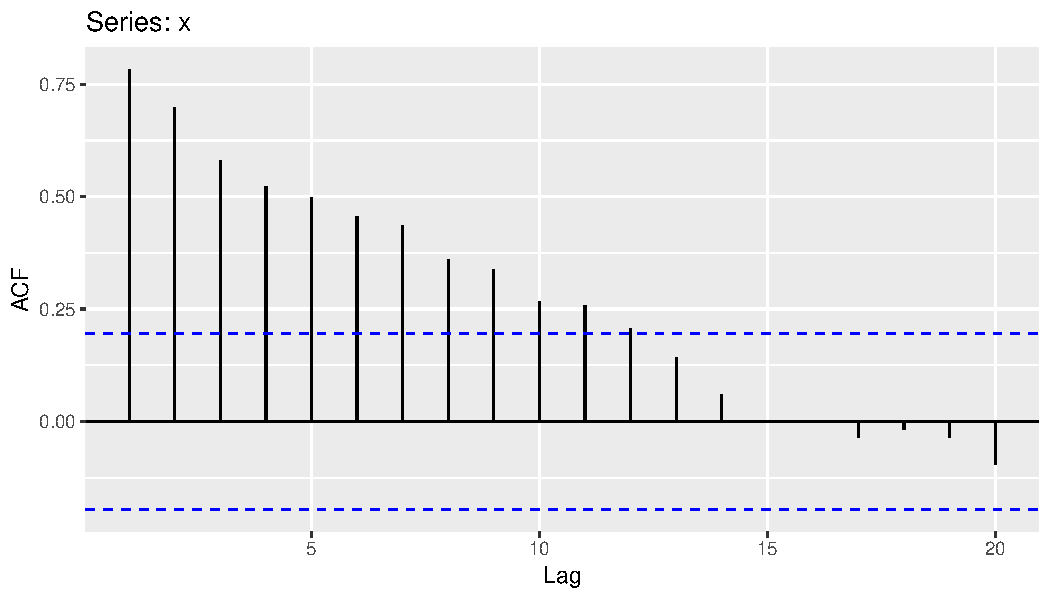
\includegraphics[width=\maxwidth]{figure/unnamed-chunk-56-1} 

\end{knitrout}
\end{frame}

\begin{frame}[fragile]{Final example: a hockey league}

  \begin{itemize}
  \item 
An Ontario hockey league has teams in 21 cities. How can we arrange those teams into 4 geographical divisions?
\item Distance data in spreadsheet.
\item Take out spaces in team names.
\item Save as ``text/csv''.
  \item Distances, so back to \texttt{hclust}.


  \end{itemize}
  
\end{frame}

\begin{frame}[fragile]{A map}

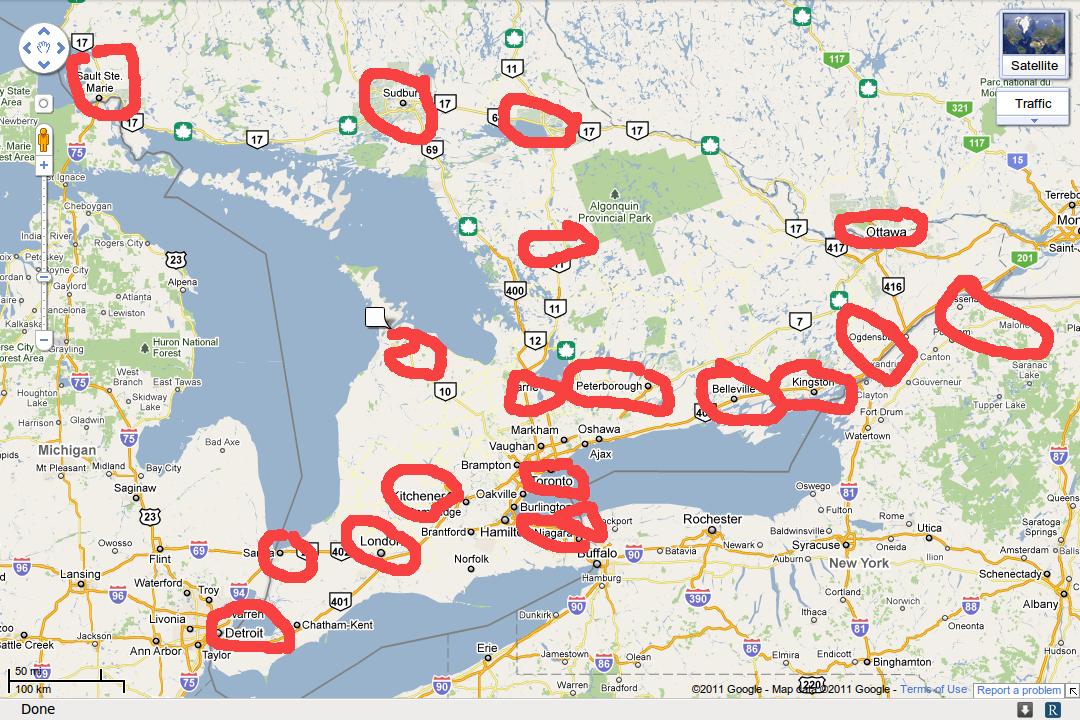
\includegraphics[width=4.5in]{map1}
\end{frame}

\begin{frame}[fragile]{Attempt 1}

  {\small
\begin{knitrout}
\definecolor{shadecolor}{rgb}{0.969, 0.969, 0.969}\color{fgcolor}\begin{kframe}
\begin{alltt}
\hlstd{ontario}\hlkwb{=}\hlkwd{read.csv}\hlstd{(}\hlstr{"ontario-road-distances.csv"}\hlstd{,}\hlkwc{header}\hlstd{=T)}
\hlstd{ontario.d}\hlkwb{=}\hlkwd{dist}\hlstd{(ontario)}
\hlstd{ontario.hc}\hlkwb{=}\hlkwd{hclust}\hlstd{(ontario.d,}\hlkwc{method}\hlstd{=}\hlstr{"ward.D"}\hlstd{)}
\hlkwd{cutree}\hlstd{(ontario.hc,}\hlnum{4}\hlstd{)}
\end{alltt}
\begin{verbatim}
##        Barrie    Belleville     Brantford 
##             1             2             1 
##    Brockville      Cornwall      Hamilton 
##             2             2             1 
##    Huntsville      Kingston     Kitchener 
##             2             2             1 
##        London  NiagaraFalls      NorthBay 
##             1             1             2 
##        Ottawa     OwenSound  Peterborough 
##             2             1             2 
##        Sarnia SaultSteMarie  StCatharines 
##             1             3             1 
##    ThunderBay       Toronto       Windsor 
##             4             1             1
\end{verbatim}
\end{kframe}
\end{knitrout}
}
  
\end{frame}

\begin{frame}[fragile]{Plot, with 4 clusters}
  
\begin{knitrout}
\definecolor{shadecolor}{rgb}{0.969, 0.969, 0.969}\color{fgcolor}\begin{kframe}
\begin{alltt}
\hlkwd{plot}\hlstd{(ontario.hc)}
\hlkwd{rect.hclust}\hlstd{(ontario.hc,}\hlnum{4}\hlstd{)}
\end{alltt}
\end{kframe}
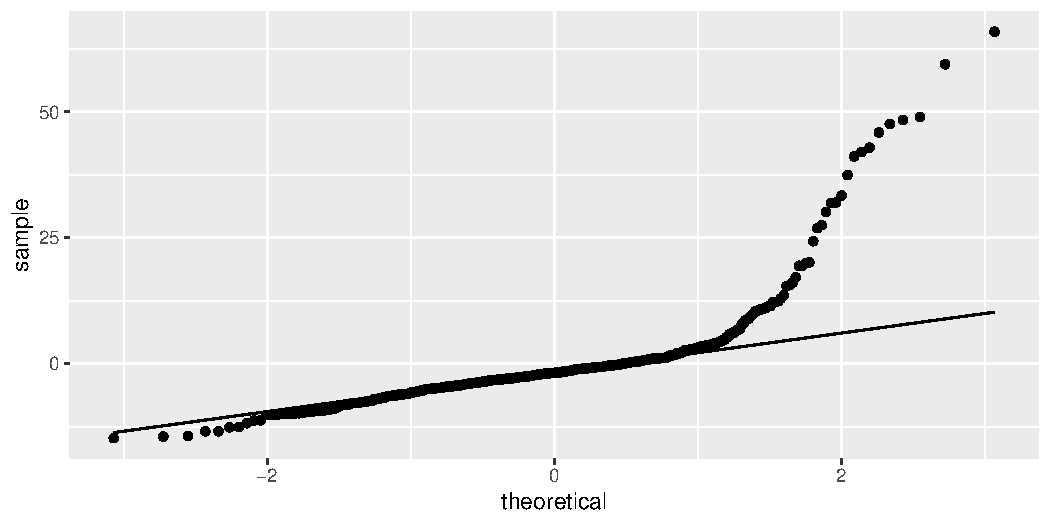
\includegraphics[width=\maxwidth]{figure/unnamed-chunk-58-1} 

\end{knitrout}
\end{frame}

\begin{frame}[fragile]{Comments}
  
  \begin{itemize}
  \item Can't have divisions of 1 team!
  \item ``Southern'' divisions way too big!
  \item Try splitting into more. I found 7 to be good:
  \end{itemize}

  
\end{frame}

\begin{frame}[fragile]{Seven clusters}
  
\begin{knitrout}
\definecolor{shadecolor}{rgb}{0.969, 0.969, 0.969}\color{fgcolor}\begin{kframe}
\begin{alltt}
\hlkwd{plot}\hlstd{(ontario.hc)}
\hlkwd{rect.hclust}\hlstd{(ontario.hc,}\hlnum{7}\hlstd{)}
\end{alltt}
\end{kframe}
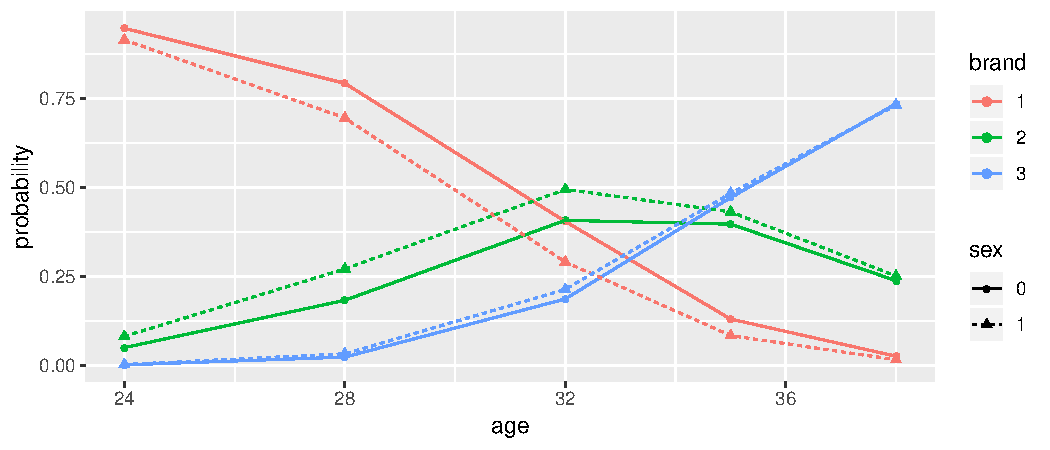
\includegraphics[width=\maxwidth]{figure/unnamed-chunk-59-1} 

\end{knitrout}
  
\end{frame}

\begin{frame}[fragile]{Divisions now}
  
  \begin{itemize}
  \item I want to put Huntsville and North Bay together with northern teams.
  \item I'll put the Eastern teams together. Gives:
    \begin{itemize}
    \item North: Sault Ste Marie, Sudbury, Huntsville, North Bay
    \item East: Brockville, Cornwall, Ottawa, Peterborough,
      Belleville, Kingston
    \item West:  Windsor, London, Sarnia
    \item Central: Owen Sound, Barrie, Toronto, Niagara Falls, St
      Catharines, Brantford, Hamilton, Kitchener
    \end{itemize}
  \item Getting them same size beyond us!
  \end{itemize}
  
\end{frame}

\begin{frame}[fragile]{Another map}

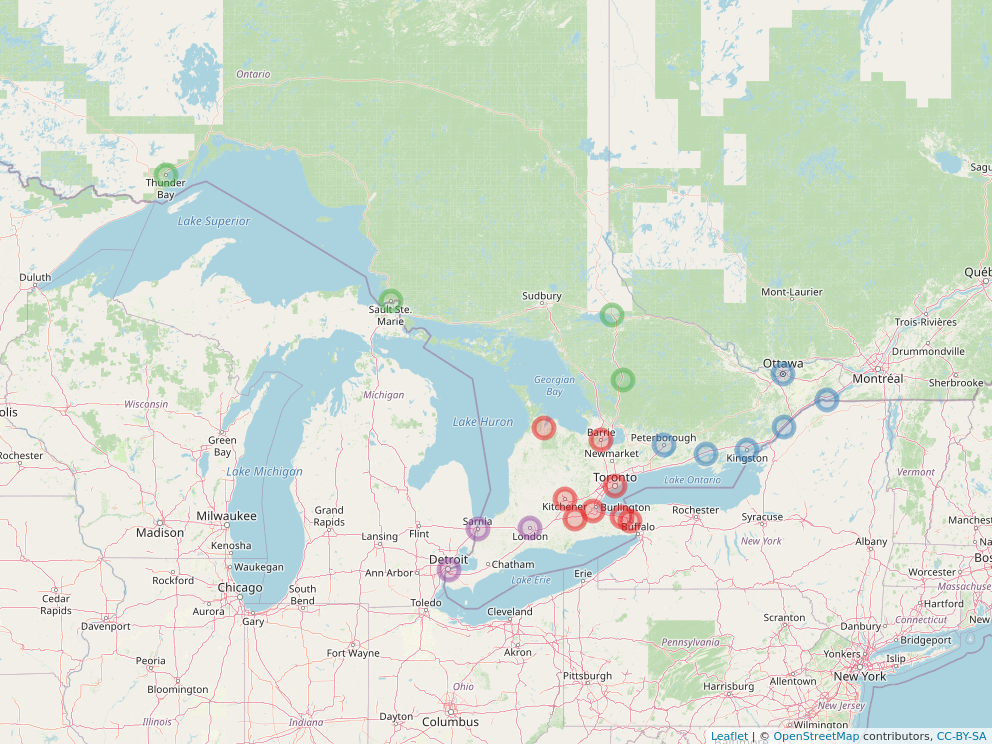
\includegraphics[width=4.5in]{map2}
  
\end{frame}

